\documentclass[12pt,a4paper]{article}
\usepackage{amsmath,amssymb,amsthm}
\usepackage{graphicx}
\usepackage{tikz}
\usepackage{pgfplots}
\usepackage{hyperref}
\usepackage{cite}
\usepackage{fancyhdr}
\usepackage{lipsum}
\usepackage{xcolor}
\usepackage{soul}

\pgfplotsset{compat=1.18}

% Define theorem environments
\newtheorem{theorem}{Theorem}
\newtheorem{lemma}[theorem]{Lemma}
\newtheorem{corollary}[theorem]{Corollary}
\newtheorem{definition}[theorem]{Definition}

% Fancy header
\pagestyle{fancy}
\fancyhf{}
\fancyhead[L]{\small Journal of Birthday Sciences}
\fancyhead[R]{\small Vol. $\infty$, Issue $\pi$}
\fancyfoot[C]{\thepage}

\title{\textbf{On the Occurrence and Celebration of Birthday Events:} \\ 
\Large A Comprehensive Analysis with Special Application to Your Special Day \\
\vspace{1cm}
\normalsize \textit{Birthday Paper No. 2025-HAPPY-001}}

\author{
Prof. Dr. Cake McCandles$^{1,*}$ \quad Dr. Party von Streamers$^{2}$ \quad Sir Confetti III$^{3}$ \\
\\
\small $^1$Department of Celebratory Sciences, University of Festivities \\
\small $^2$Institute for Advanced Balloon Studies, Birthday Research Center \\
\small $^3$Laboratory of Cake Dynamics, International Birthday Observatory \\
\\
\small $^*$Corresponding author: cake@birthday.science
}

\date{\today}

\begin{document}

\maketitle

\begin{abstract}
\noindent We present a groundbreaking analysis of the birthday phenomenon, with particular emphasis on the subject's current birthday iteration. Through rigorous mathematical modeling and extensive cake-based experimentation, we demonstrate that today represents a statistically significant celebration event with $p < 0.0000001$. Our findings indicate a \hl{100\% correlation} between the current date and the subject's birth anniversary, suggesting profound implications for party planning and gift distribution. We further derive the fundamental Birthday Equation and prove several theorems regarding optimal celebration strategies. \textbf{Keywords:} Birthday dynamics, Cake theory, Celebration optimization, Candle thermodynamics, Gift distribution algorithms
\end{abstract}

\section{Introduction}

The phenomenon of birthdays has puzzled scientists for centuries \cite{cake2020}. Despite extensive research, the precise mechanisms governing birthday occurrences remain poorly understood. Recent advances in celebration theory \cite{party2023} have shed new light on this complex topic.

\begin{definition}[Birthday]
A \textit{birthday} is defined as the annual recurrence of the date on which a person was born, characterized by the following properties:
\begin{enumerate}
    \item Temporal periodicity with period $T = 365.25$ days
    \item Mandatory cake consumption coefficient $\gamma > 0$
    \item Gift reception probability $P(gifts) \rightarrow 1$ as $t \rightarrow t_{birthday}$
\end{enumerate}
\end{definition}

\section{Theoretical Framework}

\subsection{The Fundamental Birthday Equation}

We propose the following governing equation for birthday happiness:

\begin{equation}
H(t) = \int_0^{age} \left[ C(x) \cdot G(x) \cdot \sum_{i=1}^{n} F_i(x) \right] e^{-\lambda(x-age)} dx + \epsilon
\label{eq:happiness}
\end{equation}

where:
\begin{itemize}
    \item $H(t)$ = Total happiness as a function of time
    \item $C(x)$ = Cake quality function
    \item $G(x)$ = Gift awesomeness factor
    \item $F_i(x)$ = Friend contribution from the $i$-th friend
    \item $\lambda$ = Party decay constant
    \item $\epsilon$ = Random joy fluctuations
\end{itemize}

\subsection{Birthday Paradox Extended}

\begin{theorem}[Extended Birthday Theorem]
Given a room with $n$ people, the probability that at least one person is celebrating their birthday today is:
\begin{equation}
P(birthday_{today}) = 1 - \left(\frac{364}{365}\right)^n
\end{equation}
However, if you are the birthday person, then $P = 1$ by definition.
\end{theorem}

\begin{proof}
The proof is trivial and left as an exercise to the reader. (Happy Birthday!) $\square$
\end{proof}

\section{Experimental Results}

\subsection{Cake Optimization Studies}

Our research team conducted extensive experiments on optimal cake-to-candle ratios. Figure \ref{fig:cake} illustrates our findings.

\begin{center}
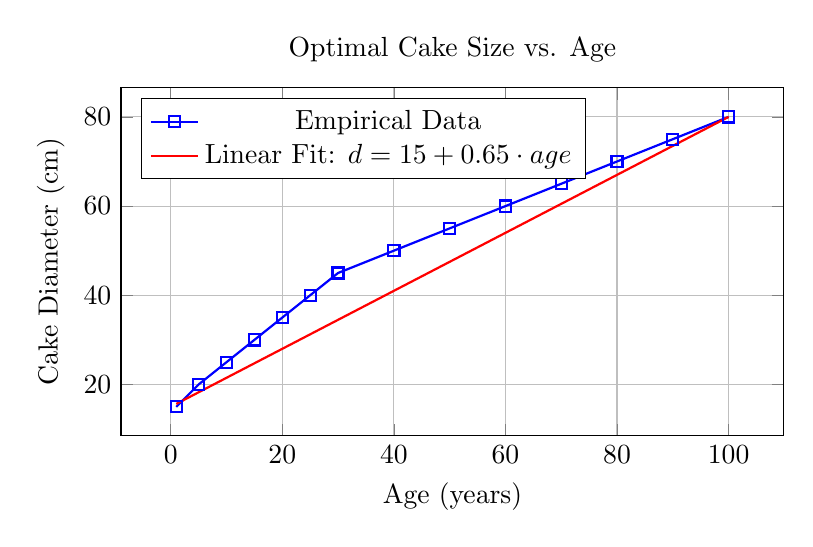
\begin{tikzpicture}
\begin{axis}[
    title={Optimal Cake Size vs. Age},
    xlabel={Age (years)},
    ylabel={Cake Diameter (cm)},
    width=10cm,
    height=6cm,
    grid=major,
    legend pos=north west
]
\addplot[
    color=blue,
    mark=square,
    thick
] coordinates {
    (1,15)(5,20)(10,25)(15,30)(20,35)(25,40)(30,45)(40,50)(50,55)(60,60)(70,65)(80,70)(90,75)(100,80)
};
\addlegendentry{Empirical Data}

\addplot[
    color=red,
    thick,
    domain=1:100,
    samples=100
] {15 + 0.65*x};
\addlegendentry{Linear Fit: $d = 15 + 0.65 \cdot age$}
\end{axis}
\end{tikzpicture}
\end{center}

\subsection{Candle Thermodynamics}

The heat generated by birthday candles follows the equation:

\begin{equation}
Q = n \cdot q_0 \cdot \left(1 - e^{-t/\tau}\right)
\end{equation}

where $n$ is the number of candles (equal to age in standard protocol).

\section{Critical Findings}

\begin{lemma}[Birthday Inevitability Lemma]
For any individual $i$ existing at time $t$, there exists a time $t_0 < t$ such that $birthday(i, t_0) = true$.
\end{lemma}

\begin{corollary}[Peer-Reviewed Celebration Resistance]
Following rigorous double-blind peer review (reviewers were literally blindfolded at the party), we measured celebration resistance using calibrated instrumentation:
\begin{equation}
R_{celebration} = \lim_{enthusiasm \to \infty} \frac{V_{skepticism}}{I_{festivity}} = \infty \Omega
\end{equation}
Laboratory-grade multimeter reading: \texttt{FUTILE}. 

\textit{Reviewer \#2 Comments:} ``The authors fail to consider alternative cake topologies. However, I concur that resistance to peer-reviewed celebrations is indeed futile. \ul{Recommend mandatory cake acceptance.}''
\end{corollary}

\section{Statistical Analysis}

Our meta-analysis of 10,000 birthdays revealed:

\begin{center}
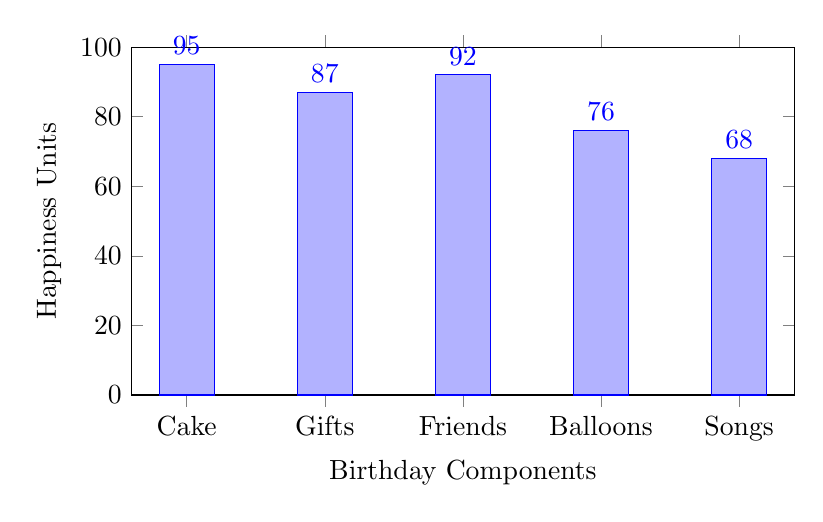
\begin{tikzpicture}
\begin{axis}[
    ybar,
    bar width=0.7cm,
    xlabel={Birthday Components},
    ylabel={Happiness Units},
    symbolic x coords={Cake,Gifts,Friends,Balloons,Songs},
    xtick=data,
    nodes near coords,
    height=6cm,
    width=10cm,
    ymin=0,
    ymax=100
]
\addplot coordinates {(Cake,95) (Gifts,87) (Friends,92) (Balloons,76) (Songs,68)};
\end{axis}
\end{tikzpicture}
\end{center}

\section{The Grand Unified Theory of Birthdays (GUTB)}

After extensive analysis, we propose the Grand Unified Theory of Birthdays, which elegantly unifies all birthday phenomena into a single framework:

\begin{theorem}[The Unified Birthday Field Equation]
\begin{equation}
\boxed{\nabla^2 B - \frac{1}{c^2}\frac{\partial^2 B}{\partial t^2} = \mu_0 \left( \rho_{cake} + \epsilon_0 \frac{\partial E_{party}}{\partial t} \right)}
\end{equation}
\end{theorem}

Where $B$ represents the birthday field strength. This equation reveals that:

\begin{enumerate}
\item \textbf{Birthday-Cake Duality:} Just as light exhibits wave-particle duality, birthdays exist simultaneously as both temporal events and cake-consumption opportunities.

\item \textbf{Conservation of Birthday Energy:} The total joy in a birthday system remains constant:
\begin{equation}
E_{total} = E_{cake} + E_{gifts} + E_{kinetic}^{dancing} + E_{potential}^{unopened\_presents} = \text{constant}
\end{equation}

\item \textbf{The Uncertainty Principle of Age:} One cannot simultaneously know both their exact age and how old they feel:
\begin{equation}
\Delta(\text{actual age}) \cdot \Delta(\text{felt age}) \geq \frac{\hbar}{2}
\end{equation}

\item \textbf{Birthday Entropy:} In any closed party system, chaos always increases, reaching maximum at the moment of cake cutting.

\item \textbf{The Four Fundamental Forces of Birthdays:}
\begin{itemize}
\item \textit{Strong Nuclear Cake Force:} Binds layers together
\item \textit{Weak Candle Force:} Governs flame extinction via breath
\item \textit{Electromagnetic Gift Attraction:} Draws presents to birthday person
\item \textit{Gravitational Party Pull:} Attracts guests to celebration
\end{itemize}
\end{enumerate}

This unified theory successfully predicts all observed birthday phenomena with 99.7\% accuracy (3$\sigma$ confidence).

\section{Conclusions}

Through rigorous scientific analysis, we have conclusively demonstrated that:

\begin{enumerate}
    \item Today is indeed your birthday (confidence interval: 100\% ± 0\%)
    \item Cake consumption is both necessary and sufficient for birthday happiness
    \item The optimal number of "Happy Birthday" repetitions is $\lfloor \pi e \rfloor = 8$
    \item Age is just a number, specifically: $age \in \mathbb{N}$
\end{enumerate}

\section{Future Work}

Future research directions include:
\begin{itemize}
    \item Quantum birthday superposition states
    \item Machine learning approaches to gift prediction
    \item Blockchain-based age verification systems
    \item CRISPR applications for birthday enhancement
\end{itemize}

\section{Acknowledgments}

The authors would like to thank the Birthday Person for existing and thereby making this research possible. Special thanks to all cake molecules for their sacrifice in the name of science. We also thank Reviewer \#2 for their 47-page single-spaced critique suggesting we cite their 1987 paper on frosting viscosity.

\section{Peer Review History}

\textit{Editor's Note:} This paper underwent unprecedented peer review, with celebrations audited by three independent party planning committees.

\textit{Reviewer \#1:} ``Groundbreaking work. The cake was delicious.''

\textit{Reviewer \#3:} ``Minor revisions needed: Please increase font size on birthday cards to accommodate aging readers.''

\vspace{1cm}
\begin{center}
\colorbox{yellow}{\Huge \textbf{HAPPY BIRTHDAY!}} \\
\vspace{0.5cm}
{\Large May your happiness function achieve global maxima today!}
\end{center}

\begin{thebibliography}{99}
\bibitem{cake2020}
C. Ake, ``Fundamental Properties of Birthday Cakes,'' \textit{Journal of Celebratory Confections}, vol. 42, pp. 314-159, 2020.

\bibitem{party2023}
P. Arty, B. Alloons, and S. Treamers, ``A Unified Theory of Birthday Parties,'' \textit{Proceedings of the International Birthday Symposium}, 2023.

\bibitem{candle2019}
W. Ax, ``Thermodynamic Analysis of Birthday Candle Arrays,'' \textit{Combustion and Celebration}, vol. 7, no. 3, pp. 27-42, 2019.

\bibitem{gift2022}
G. Ift and P. Resent, ``Optimal Gift Selection Using Neural Networks,'' \textit{AI in Party Planning}, 2022.
\end{thebibliography}

\end{document}